\newpage
\begin{tcolorbox}
\chapter{2015 - Pivo Moz}
		\lettrine{W}{ith} 2.2 km discovered in \passage{Vrtnarija}, all below 600 m, Pivo Moz 2015 was another successful year of deep pushing. Significant work went into the extensions off \passage{Sic Semper Tyrannis} which led to the closure of an 840m loop in the south, while \passage{Colarado Duck} was passed with a further 270m of passage found beyond. Aven climbing at \passage{Strap on the Nitro} enabled the discovery of 294 m of south trending passage heading towards \passage{Wonderstuff} in the ‘old system’. 

		For the first time in \passage{Migovec} exploration two underground camps were operational at the same time:\passage{Camp X-Ray} at -650 m, a 4 berth camp set up in a central position, and \passage{Camp Deep Core II} at -850 m near \passage{Red Cow}, a 2 berth camp set up by divers Jarvist Frost and Connor Roe for future use as access to the \passage{Watership Down} sump, and used this year by them as a staging post for the northern extensions. \passage{Camp X-Ray} remained the main exploration camp. All leads however were then more than 2.5 hours away, raising the possibility of setting up another camp, closer to the southern leads in \passage{Sic Semper Tyrannis}.
	

\end{tcolorbox}
	\backgroundsetup{	scale=1,
					color=black,
					opacity=1,
					angle=0,
					contents={%
 							 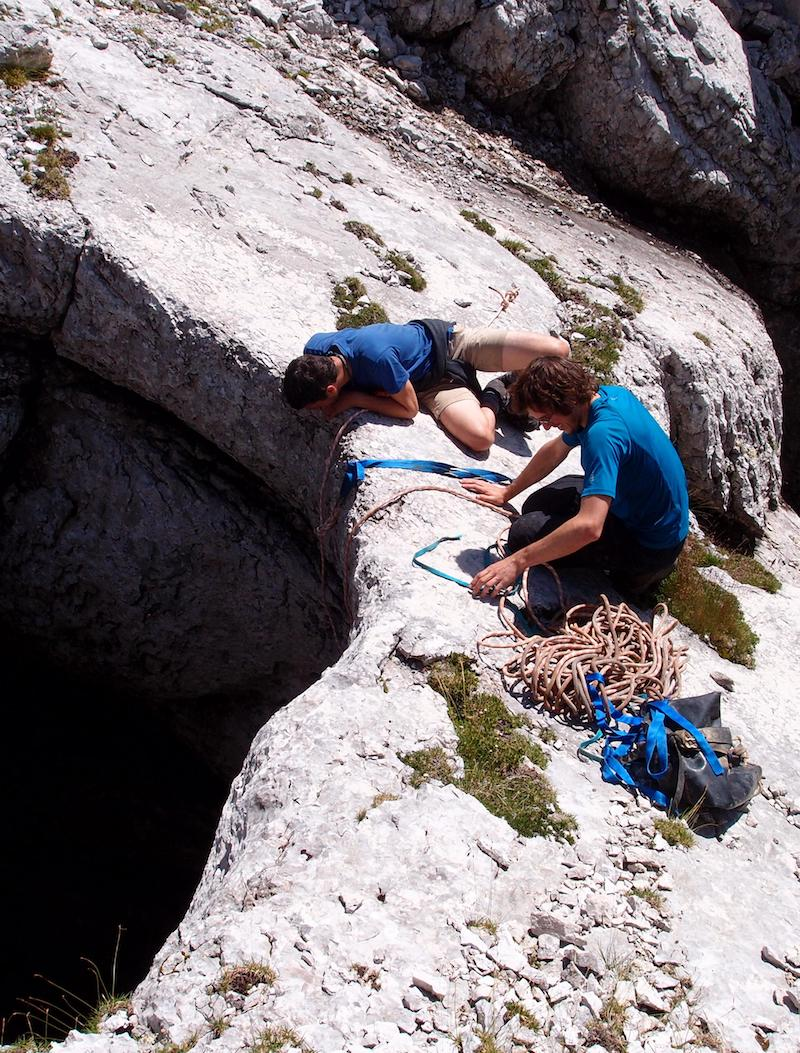
\includegraphics[height=\paperheight]{images/backgrounds/surfacepothole.jpg}
  					}
	}
\BgThispage



